% Drawing 147/04-4 -- folder 147, batch 04, archive page 69 (PDF page 70).
% Transcription: tableau à trois colonnes. Codimension 1 : $G_0$ est une boucle fermée sur un sommet épais marqué $I(2)$ ; $G_1$ un segment joignant un sommet marqué 1 à un sommet marqué $I(2)$. Codimension 2 : $P_0$, deux sommets marqués $\{a\}$ et $\{b\}$ joints par deux arêtes ; $P_1$, une boucle portée par un sommet relié par une arête à un sommet marqué $I(2)$. Des flèches vont de $G_0$ vers $P_0$ (marquée 2) et vers $P_1$ (marquée 1), et de $G_1$ vers $P_1$ (marquée 1)
% Kind: table of MD graphs by codimension, with degeneration arrows. Method 3 (encoded, rendered from the data). Status: ok.
% Notes: Table (83) for hat M^!_{1,2}: codim 0, a vertex of genus 1 with I(2); codim 1, G_0 (loop on a thick vertex I(2)) and G_1 (segment from a vertex marked 1 = genus 1 to a vertex I(2)); codim 2, P_0 (vertices {a}, {b} joined by two edges) and P_1 (loop on a vertex joined to a vertex I(2)). Arrows G_0 -> P_0 (marked 2), G_0 -> P_1 (1), G_1 -> P_1 (1). Encoded as stable graphs: all five are of type (1,2), and their stratum dimensions 2, 1, 1, 0, 0 match the column codimensions 0, 1, 1, 2, 2. The arrows (specialisations) are not encoded.
% Coordinates: 1 unit = 1 mm = 1/100 of the crop width (bbox in page fractions: [0.266, 0.14, 0.804, 0.271]).
% Redrawn by Claude (claude-opus-5-5), issue #73, 2026-11-07; not checked by a human; not compiled (no TeX in the session).
% Rights: reproduces part of the work -- behind RENDER_TRANSCRIPTS, never published by itself.
\documentclass[tikz,border=3pt]{standalone}
\usepackage{amsmath,amssymb}
\usetikzlibrary{patterns,arrows.meta}
\tikzset{pencil/.style={black!45}, struck/.style={black!35}, mark/.style={circle,draw,inner sep=1.3pt}, pt/.style={circle,fill,inner sep=0.9pt}, opt/.style={circle,draw,fill=white,inner sep=1.1pt}}
\begin{document}
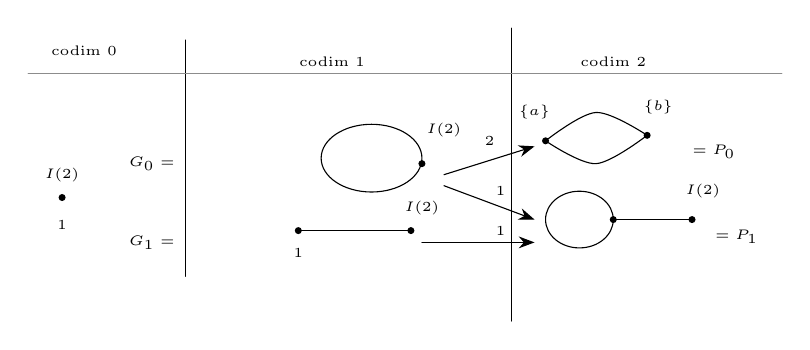
\begin{tikzpicture}[x=1mm,y=1mm,line cap=round,line join=round,font=\scriptsize]
\draw (24.3,-2.9) -- (24.3,-32.9);
\draw (65.7,-1.4) -- (65.7,-38.6);
\draw[pencil] (4.3,-7.1) -- (100,-7.1);
\node[inner sep=1pt] at (11.4,-4.3) {\tiny codim 0};
\node[inner sep=1pt] at (42.9,-5.7) {\tiny codim 1};
\node[inner sep=1pt] at (78.6,-5.7) {\tiny codim 2};
\node[pt] at (8.6,-22.9) {};
\node[inner sep=1pt] at (8.6,-20) {\tiny $I(2)$};
\node[inner sep=1pt] at (8.6,-26.4) {\tiny $1$};
\node[inner sep=1pt] at (20,-18.6) {\tiny $G_0=$};
\draw (47.9,-17.9) ellipse[x radius=6.4, y radius=4.3];
\node[pt,very thick] at (54.3,-18.6) {};
\node[inner sep=1pt] at (57.1,-14.3) {\tiny $I(2)$};
\node[inner sep=1pt] at (20,-28.6) {\tiny $G_1=$};
\draw (38.6,-27.1) -- (52.9,-27.1);
\node[pt] at (38.6,-27.1) {};
\node[pt] at (52.9,-27.1) {};
\node[inner sep=1pt] at (38.6,-30) {\tiny $1$};
\node[inner sep=1pt] at (54.3,-24.3) {\tiny $I(2)$};
\node[pt] at (70,-15.7) {};
\node[pt] at (82.9,-15) {};
\draw plot[smooth, tension=0.55] coordinates {(70,-15.7) (76.4,-12.1) (82.9,-15)};
\draw plot[smooth, tension=0.55] coordinates {(70,-15.7) (76.4,-18.6) (82.9,-15)};
\node[inner sep=1pt] at (68.6,-12.1) {\tiny $\{a\}$};
\node[inner sep=1pt] at (84.3,-11.4) {\tiny $\{b\}$};
\node[inner sep=1pt] at (91.4,-17.1) {\tiny $=P_0$};
\draw (74.3,-25.7) ellipse[x radius=4.3, y radius=3.6];
\node[pt] at (78.6,-25.7) {};
\draw (78.6,-25.7) -- (88.6,-25.7);
\node[pt] at (88.6,-25.7) {};
\node[inner sep=1pt] at (90,-22.1) {\tiny $I(2)$};
\node[inner sep=1pt] at (94.3,-27.9) {\tiny $=P_1$};
\draw[-{Stealth[length=2mm]}] (57.1,-20) -- (68.6,-16.4);
\node[inner sep=1pt] at (62.9,-15.7) {\tiny $2$};
\draw[-{Stealth[length=2mm]}] (57.1,-21.4) -- (68.6,-25.7);
\node[inner sep=1pt] at (64.3,-22.1) {\tiny $1$};
\draw[-{Stealth[length=2mm]}] (54.3,-28.6) -- (68.6,-28.6);
\node[inner sep=1pt] at (64.3,-27.1) {\tiny $1$};
\end{tikzpicture}
\end{document}
